% Created by tikzDevice version 0.12.3.1 on 2022-09-02 13:44:16
% !TEX encoding = UTF-8 Unicode
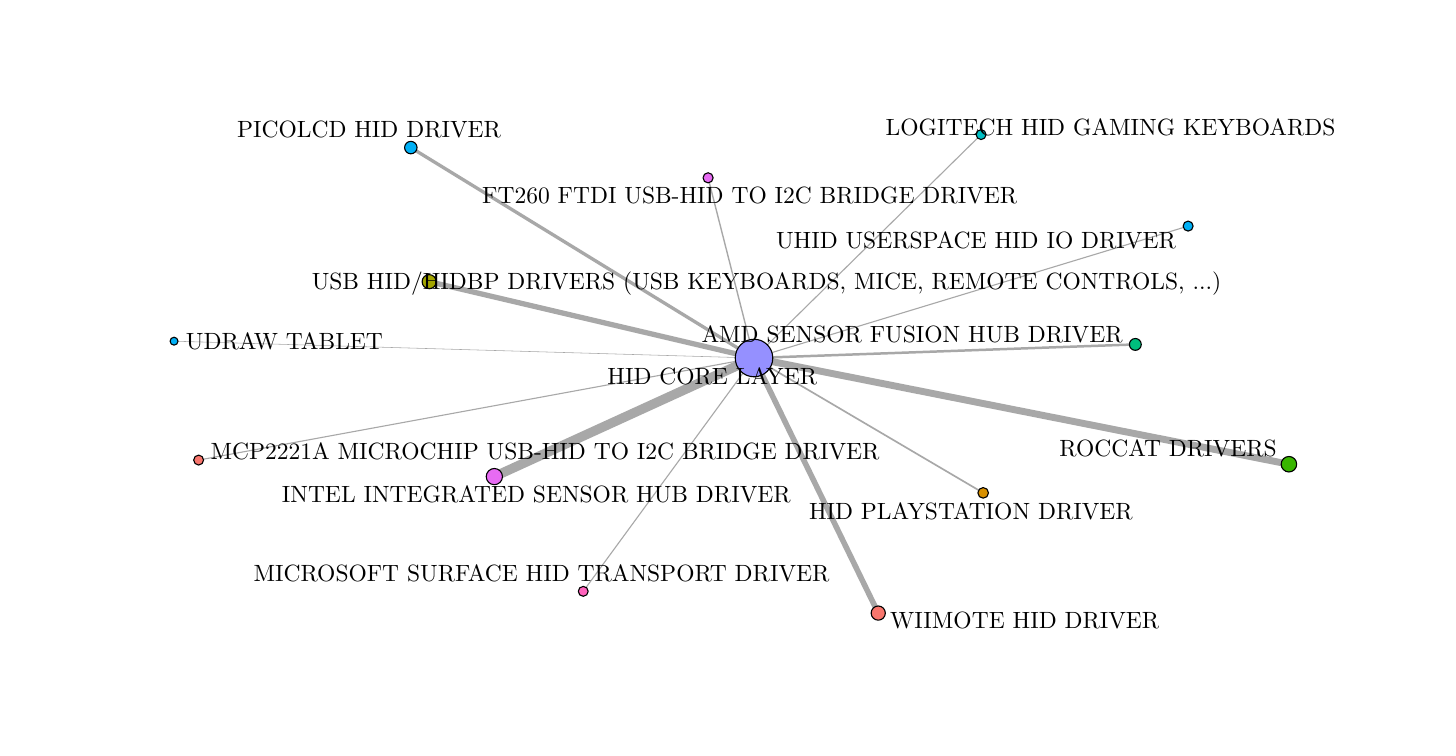
\begin{tikzpicture}[x=1pt,y=1pt]
\definecolor{fillColor}{RGB}{255,255,255}
\path[use as bounding box,fill=fillColor,fill opacity=0.00] (0,0) rectangle (505.89,252.94);
\begin{scope}
\path[clip] (  0.00,  0.00) rectangle (505.89,252.94);
\definecolor{fillColor}{RGB}{255,255,255}

\path[fill=fillColor] (  0.00,  0.00) rectangle (505.89,252.94);
\end{scope}
\begin{scope}
\path[clip] ( 32.75, 32.75) rectangle (475.89,222.94);
\definecolor{drawColor}{gray}{0.66}

\path[draw=drawColor,line width= 0.9pt,line join=round] (400.25,138.48) -- (262.46,133.57);

\path[draw=drawColor,line width= 0.5pt,line join=round] (245.86,198.68) -- (262.46,133.57);

\path[draw=drawColor,line width= 0.6pt,line join=round] (262.46,133.57) -- (345.27, 84.84);

\path[draw=drawColor,line width= 3.4pt,line join=round] (262.46,133.57) -- (168.63, 90.72);

\path[draw=drawColor,line width= 0.4pt,line join=round] (262.46,133.57) -- (344.51,214.30);

\path[draw=drawColor,line width= 0.4pt,line join=round] (262.46,133.57) -- ( 61.77, 96.69);

\path[draw=drawColor,line width= 0.4pt,line join=round] (262.46,133.57) -- (200.75, 49.26);

\path[draw=drawColor,line width= 1.2pt,line join=round] (262.46,133.57) -- (138.45,209.61);

\path[draw=drawColor,line width= 2.5pt,line join=round] (262.46,133.57) -- (455.75, 95.19);

\path[draw=drawColor,line width= 0.2pt,line join=round] (262.46,133.57) -- ( 52.89,139.65);

\path[draw=drawColor,line width= 0.4pt,line join=round] (262.46,133.57) -- (419.32,181.24);

\path[draw=drawColor,line width= 1.9pt,line join=round] (262.46,133.57) -- (145.08,161.16);

\path[draw=drawColor,line width= 2.0pt,line join=round] (262.46,133.57) -- (307.35, 41.40);
\definecolor{drawColor}{RGB}{0,0,0}
\definecolor{fillColor}{RGB}{0,191,125}

\path[draw=drawColor,line width= 0.4pt,line join=round,line cap=round,fill=fillColor] (400.25,138.48) circle (  2.14);
\definecolor{fillColor}{RGB}{231,107,243}

\path[draw=drawColor,line width= 0.4pt,line join=round,line cap=round,fill=fillColor] (245.86,198.68) circle (  1.83);
\definecolor{fillColor}{RGB}{149,144,255}

\path[draw=drawColor,line width= 0.4pt,line join=round,line cap=round,fill=fillColor] (262.46,133.57) circle (  6.78);
\definecolor{fillColor}{RGB}{216,144,0}

\path[draw=drawColor,line width= 0.4pt,line join=round,line cap=round,fill=fillColor] (345.27, 84.84) circle (  1.92);
\definecolor{fillColor}{RGB}{231,107,243}

\path[draw=drawColor,line width= 0.4pt,line join=round,line cap=round,fill=fillColor] (168.63, 90.72) circle (  2.93);
\definecolor{fillColor}{RGB}{0,191,196}

\path[draw=drawColor,line width= 0.4pt,line join=round,line cap=round,fill=fillColor] (344.51,214.30) circle (  1.79);
\definecolor{fillColor}{RGB}{248,118,109}

\path[draw=drawColor,line width= 0.4pt,line join=round,line cap=round,fill=fillColor] ( 61.77, 96.69) circle (  1.79);
\definecolor{fillColor}{RGB}{255,98,188}

\path[draw=drawColor,line width= 0.4pt,line join=round,line cap=round,fill=fillColor] (200.75, 49.26) circle (  1.79);
\definecolor{fillColor}{RGB}{0,176,246}

\path[draw=drawColor,line width= 0.4pt,line join=round,line cap=round,fill=fillColor] (138.45,209.61) circle (  2.25);
\definecolor{fillColor}{RGB}{57,182,0}

\path[draw=drawColor,line width= 0.4pt,line join=round,line cap=round,fill=fillColor] (455.75, 95.19) circle (  2.80);
\definecolor{fillColor}{RGB}{0,176,246}

\path[draw=drawColor,line width= 0.4pt,line join=round,line cap=round,fill=fillColor] ( 52.89,139.65) circle (  1.43);

\path[draw=drawColor,line width= 0.4pt,line join=round,line cap=round,fill=fillColor] (419.32,181.24) circle (  1.81);
\definecolor{fillColor}{RGB}{163,165,0}

\path[draw=drawColor,line width= 0.4pt,line join=round,line cap=round,fill=fillColor] (145.08,161.16) circle (  2.55);
\definecolor{fillColor}{RGB}{248,118,109}

\path[draw=drawColor,line width= 0.4pt,line join=round,line cap=round,fill=fillColor] (307.35, 41.40) circle (  2.56);

\node[text=drawColor,anchor=base,inner sep=0pt, outer sep=0pt, scale=  0.85] at (319.59,139.25) {AMD SENSOR FUSION HUB DRIVER};

\node[text=drawColor,anchor=base,inner sep=0pt, outer sep=0pt, scale=  0.85] at (260.92,189.27) {FT260 FTDI USB-HID TO I2C BRIDGE DRIVER};

\node[text=drawColor,anchor=base,inner sep=0pt, outer sep=0pt, scale=  0.85] at (247.39,124.15) {HID CORE LAYER};

\node[text=drawColor,anchor=base,inner sep=0pt, outer sep=0pt, scale=  0.85] at (340.83, 75.38) {HID PLAYSTATION DRIVER};

\node[text=drawColor,anchor=base,inner sep=0pt, outer sep=0pt, scale=  0.85] at (183.79, 81.25) {INTEL INTEGRATED SENSOR HUB DRIVER};

\node[text=drawColor,anchor=base,inner sep=0pt, outer sep=0pt, scale=  0.85] at (391.30,214.05) {LOGITECH HID GAMING KEYBOARDS};

\node[text=drawColor,anchor=base,inner sep=0pt, outer sep=0pt, scale=  0.85] at (186.95, 97.06) {MCP2221A MICROCHIP USB-HID TO I2C BRIDGE DRIVER};

\node[text=drawColor,anchor=base,inner sep=0pt, outer sep=0pt, scale=  0.85] at (185.67, 52.80) {MICROSOFT SURFACE HID TRANSPORT DRIVER};

\node[text=drawColor,anchor=base,inner sep=0pt, outer sep=0pt, scale=  0.85] at (123.36,213.15) {PICOLCD HID DRIVER};

\node[text=drawColor,anchor=base,inner sep=0pt, outer sep=0pt, scale=  0.85] at (412.08, 97.83) {ROCCAT DRIVERS};

\node[text=drawColor,anchor=base,inner sep=0pt, outer sep=0pt, scale=  0.85] at ( 92.79,136.72) {UDRAW TABLET};

\node[text=drawColor,anchor=base,inner sep=0pt, outer sep=0pt, scale=  0.85] at (342.66,173.03) {UHID USERSPACE HID IO DRIVER};

\node[text=drawColor,anchor=base,inner sep=0pt, outer sep=0pt, scale=  0.85] at (266.99,158.22) {USB HID/HIDBP DRIVERS (USB KEYBOARDS, MICE, REMOTE CONTROLS, ...)};

\node[text=drawColor,anchor=base,inner sep=0pt, outer sep=0pt, scale=  0.85] at (360.28, 35.77) {WIIMOTE HID DRIVER};
\end{scope}
\end{tikzpicture}
